\subsection{Scaling the agent increases performance}
\label{sec:scaling_results}

\begin{figure}[t!]
    \centering
    \begin{subfigure}[b]{0.49\textwidth}
        \centering
        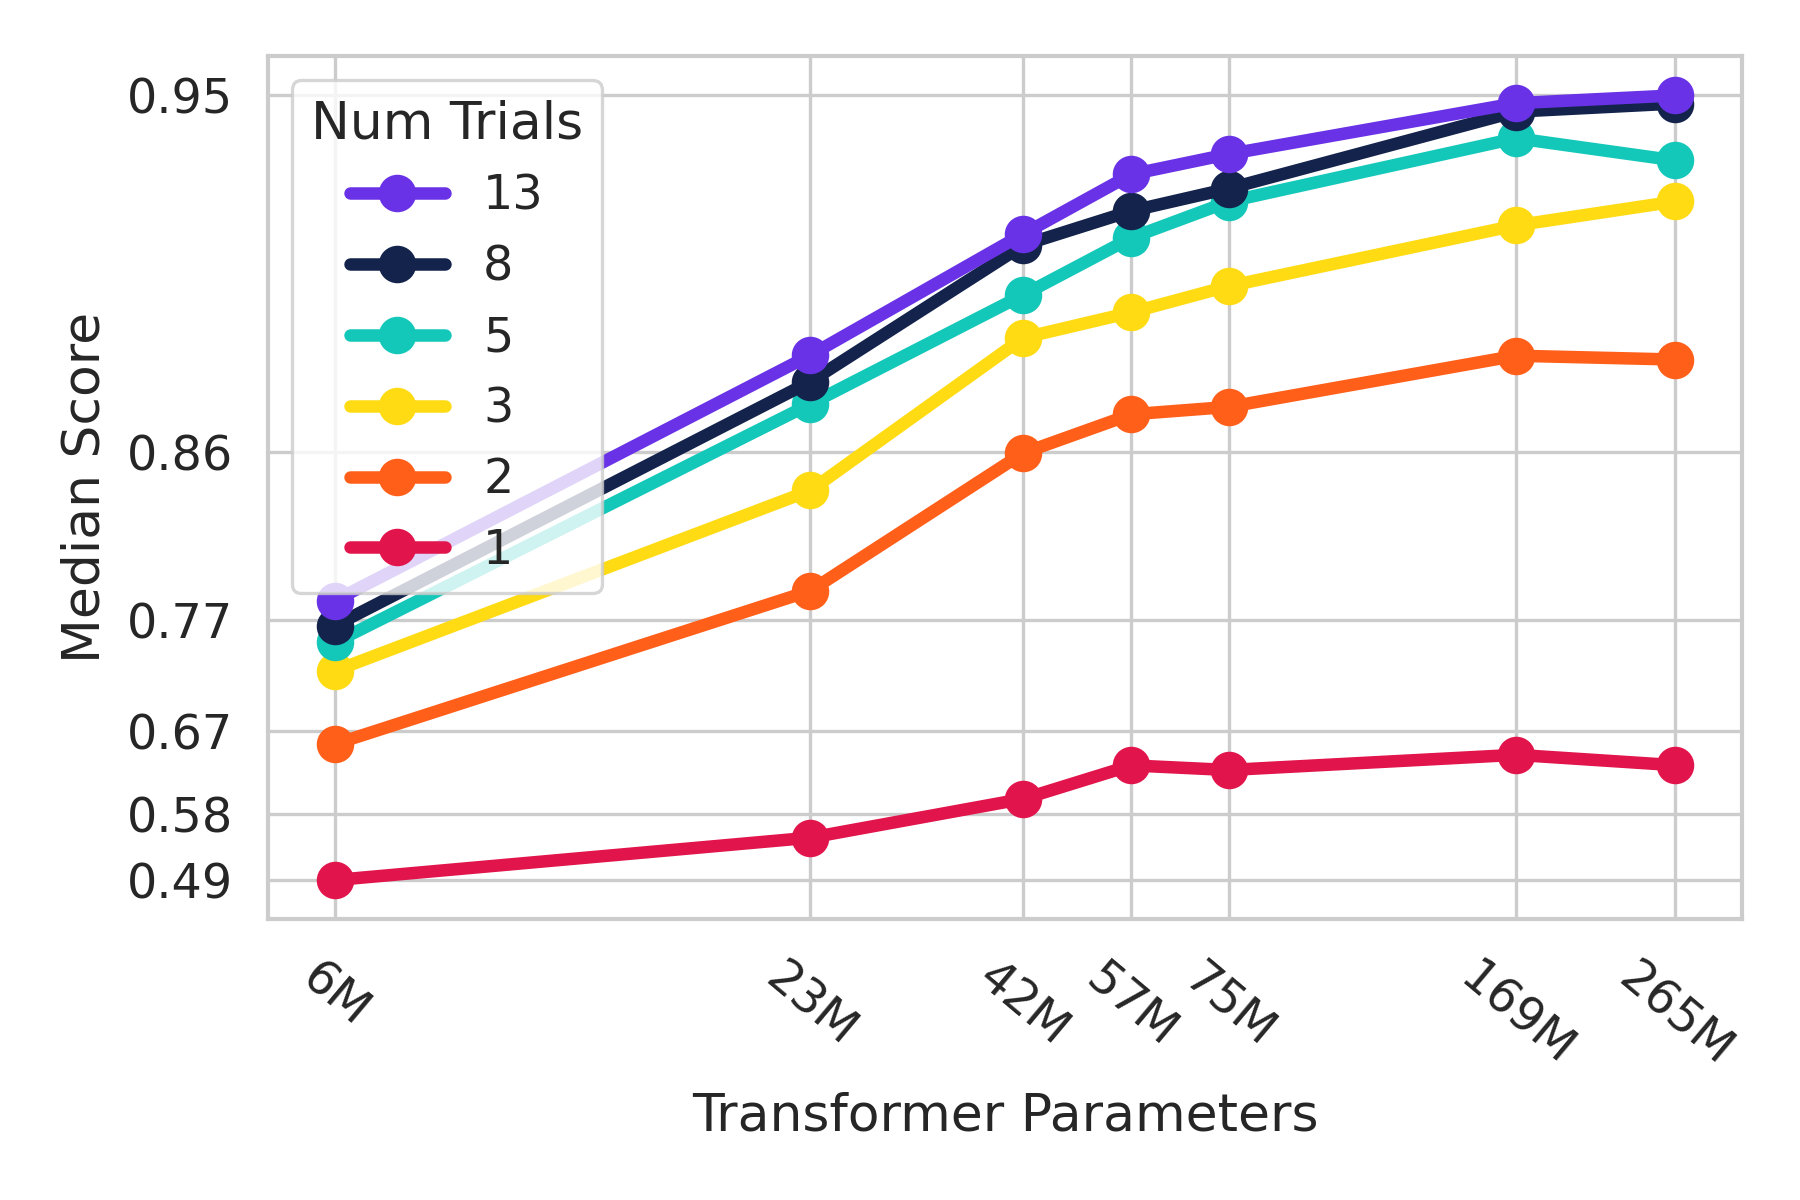
\includegraphics[width=\linewidth]{figures/scaling/parameter_scaling_75g_steps_percentile50_log_log_transformer_parameters.png}
        \vskip -3pt \caption{}
        \label{figure:scaling_network_50th}
    \end{subfigure}
    \begin{subfigure}[b]{0.49\textwidth}
        \centering
        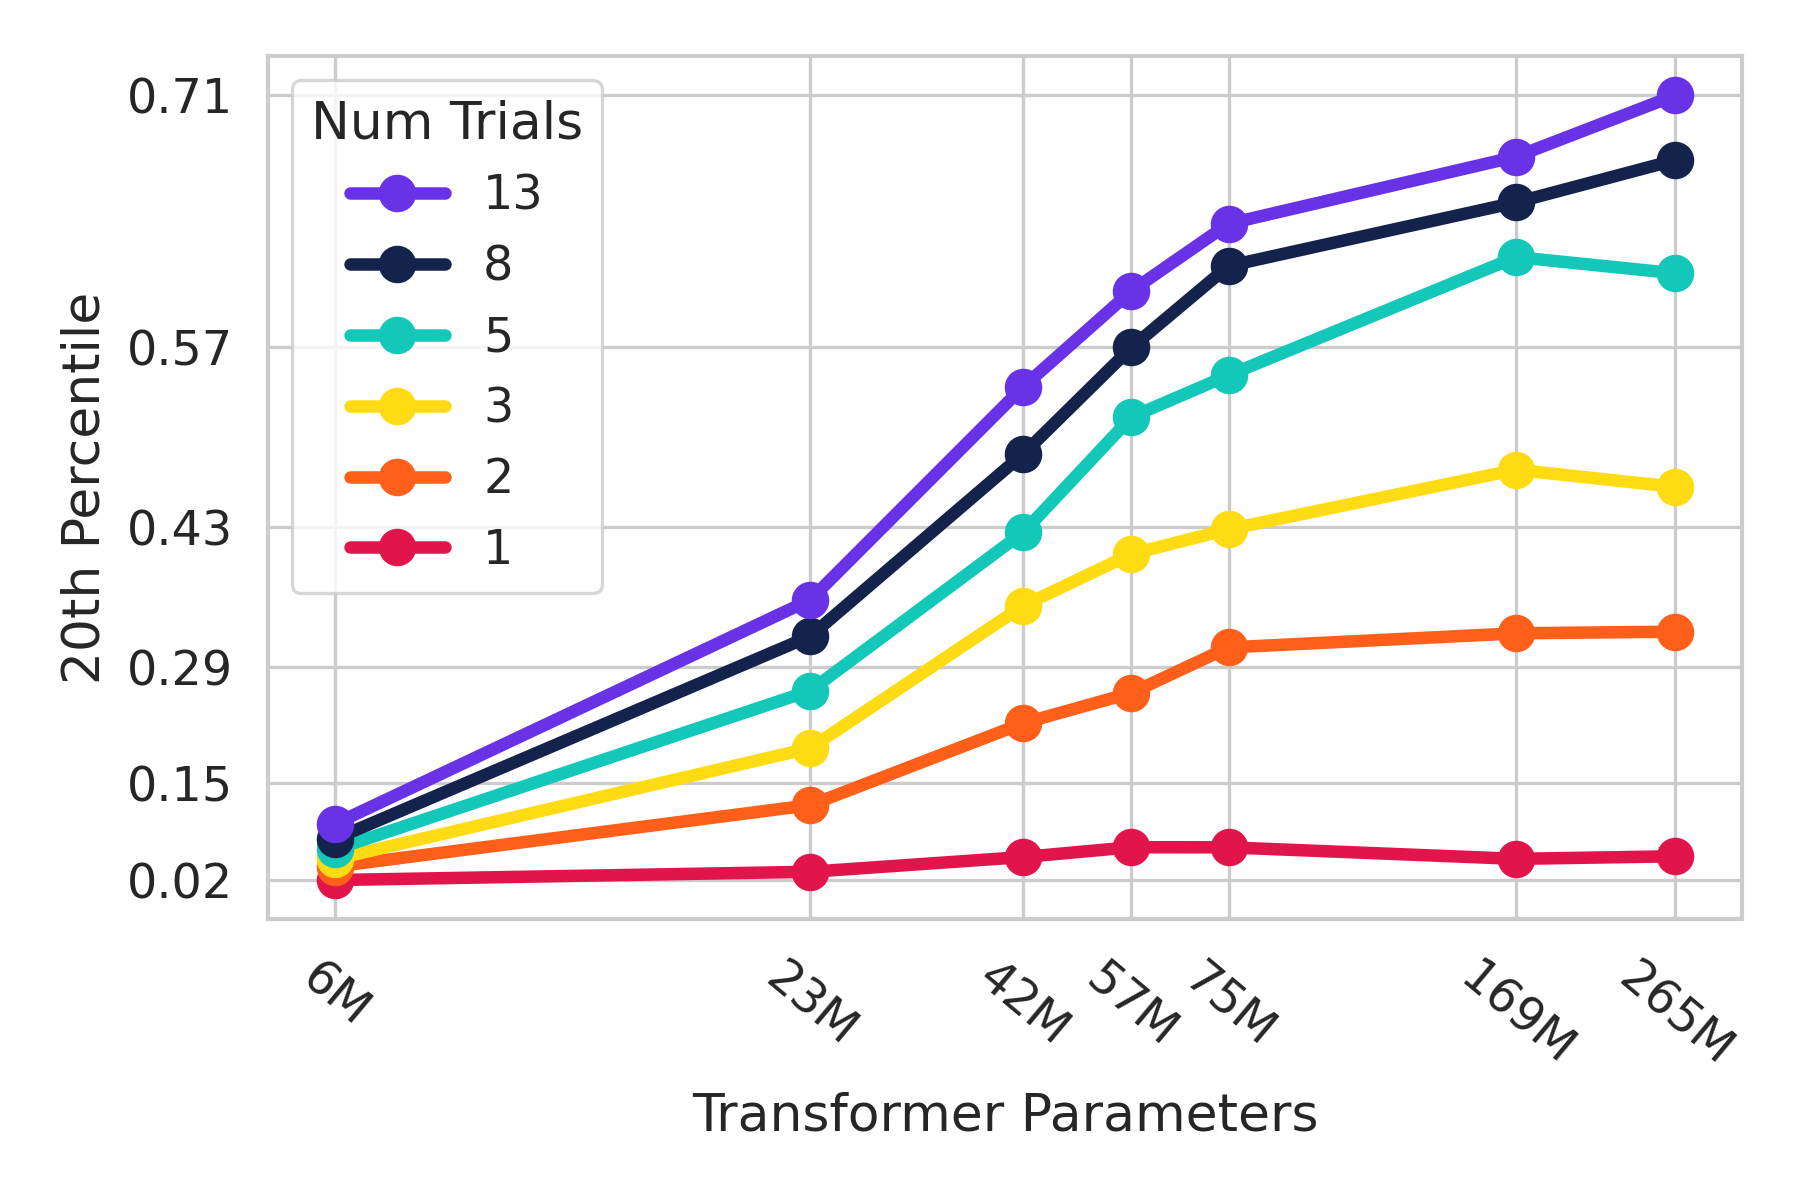
\includegraphics[width=\linewidth]{figures/scaling/parameter_scaling_75g_steps_percentile20_log_log_transformer_parameters.png}
        \vskip -3pt \caption{}
        \label{figure:scaling_network_20th}
    \end{subfigure}
    \caption{Scaling Transformer parameters increases 
    both median \textbf{(a)} and 20th percentile \textbf{(b)} test score. Both axes are log-scaled, according to the functions $\log(x)$ and $-\log(1-y)$, respectively, and the relationship between model size and performance appears roughly linear on this scale. The slope is steeper when evaluating higher numbers of trials, showing that scaling the model is particularly effective at encouraging stronger adaptation, as opposed to stronger zero-shot generalisation.}
\label{figure:scaling_network}
\end{figure}

Methods that scale well are critical for continued progress in machine learning, and understanding how methods scale is important for deciding where to spend time and compute in the future. Scaling laws have been determined for many foundation models (see Section \ref{sec:related_work}), where performance is related to model size and other factors as a power law, which can be seen as a linear relationship on a log-log plot. Inspired by such analyses, we investigate how adaptation scales with Transformer model size and memory length.

\paragraph{Scaling network size.}

We show how performance scales with the size of AdA's Transformer model, experimenting with the model sizes shown in Table \ref{tab:model_scaling}. When investigating scaling laws for model size, we follow \citet{kaplan2020scaling} in measuring only Transformer (i.e. non-embedding) parameters, which range across $3$ orders of magnitude, from $6$M to $265$M Transformer parameters (i.e. from $41$M to $533$M total parameters). A complete list of hyperparameters is shown in Table \ref{tab:model_hparams}.

Figure \ref{figure:scaling_network} shows that larger networks increase performance, especially when given more test-time trials to adapt. Though larger models seem to help in the median test-set score (Figure \ref{figure:scaling_network_50th}), model scale particularly has impact on the lower percentiles of the test set (Figure \ref{figure:scaling_network_20th}). This indicates that larger models allow the agent to generalise its adaptation to a broader range of tasks. 
The roughly linear relationship between model size and performance on the log-log plot is indicative of a power law scaling relationship, albeit only shown across two to three orders of magnitude. That the curves are not exactly linear may be due to several factors: that we haven't trained to convergence (though performance increases had slowed for all models), and that we use a 23M parameter distillation teacher across experiments for all model sizes. 

\begin{figure}[t!]
    \centering
    \begin{subfigure}[b]{0.49\textwidth}
        \centering
        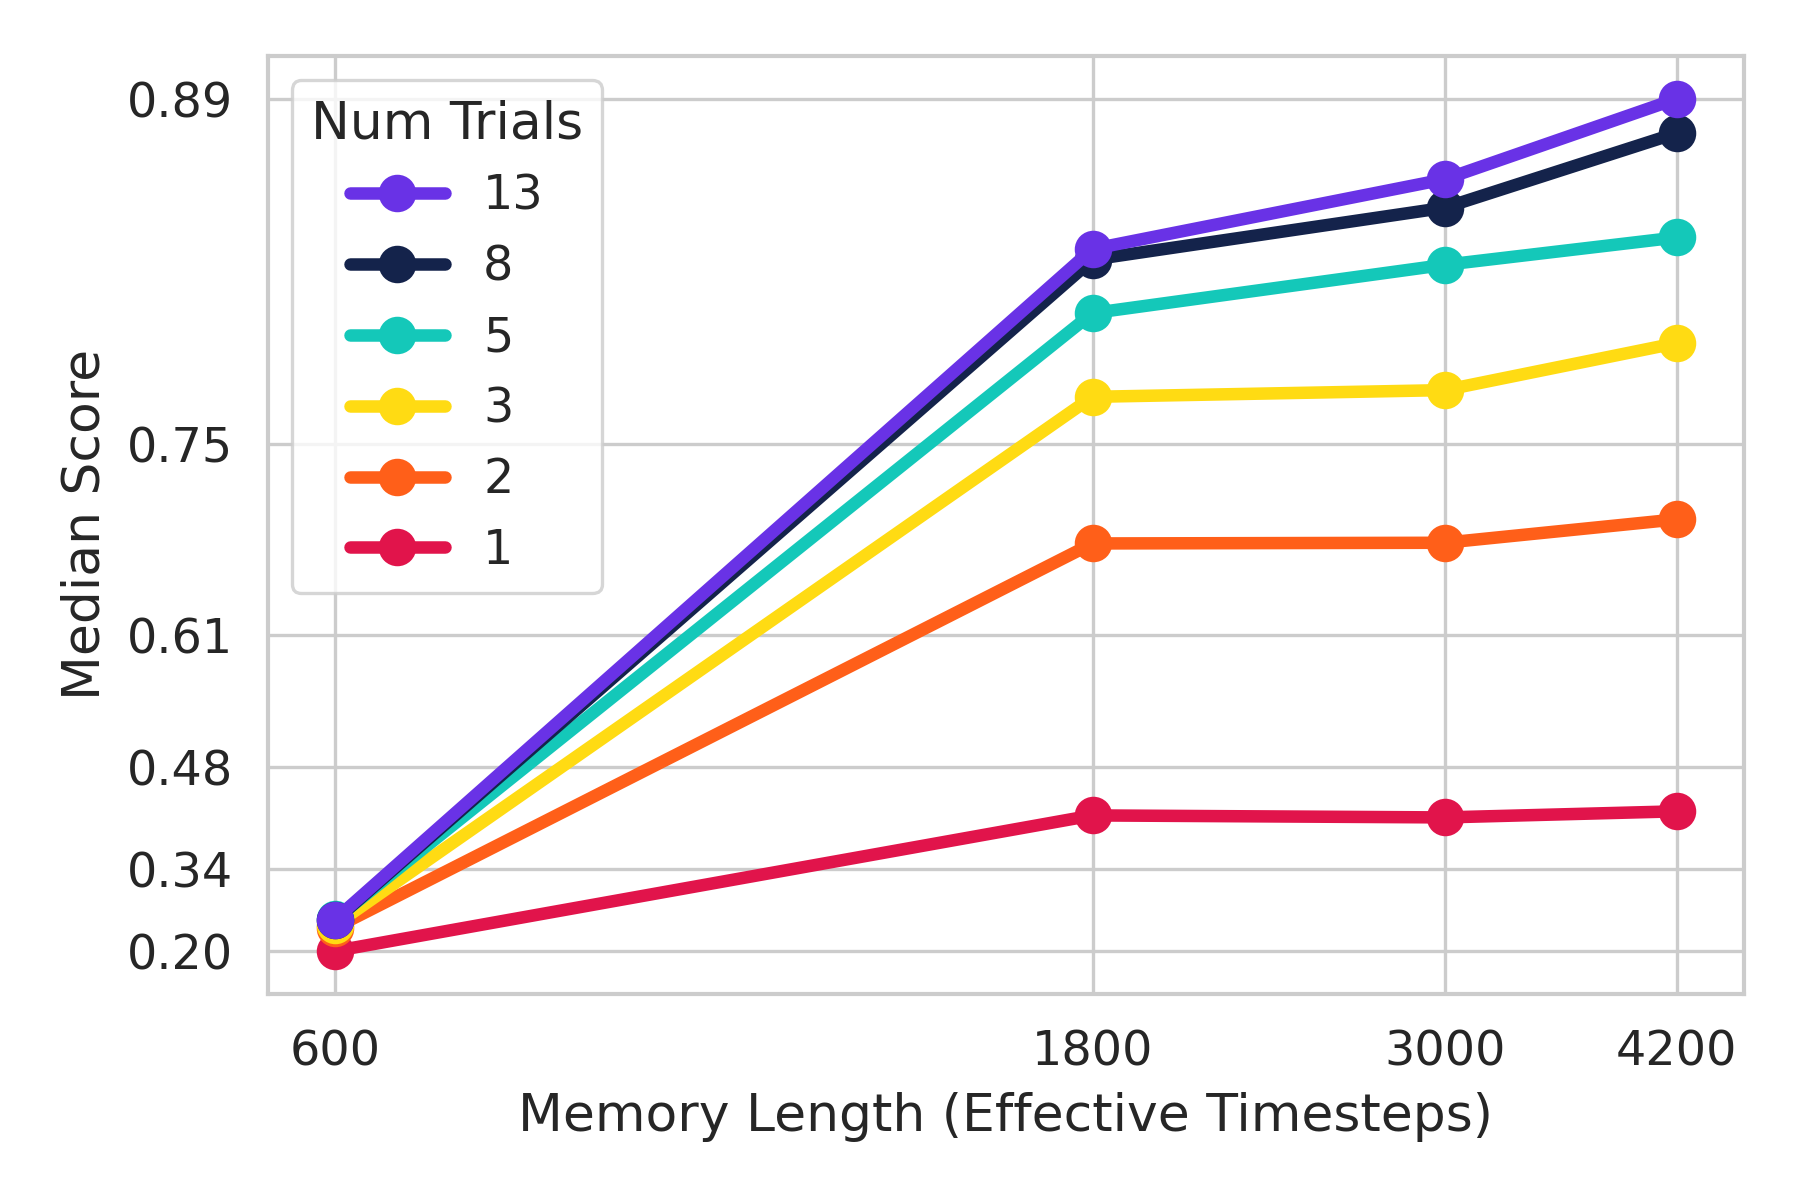
\includegraphics[width=\linewidth]{figures/scaling/memory_scaling_25g_steps_percentile50_log_log_memory.png}
        \vskip -3pt \caption{}
        \label{figure:scaling_memory_50th}
    \end{subfigure}
    \begin{subfigure}[b]{0.49\textwidth}
        \centering
        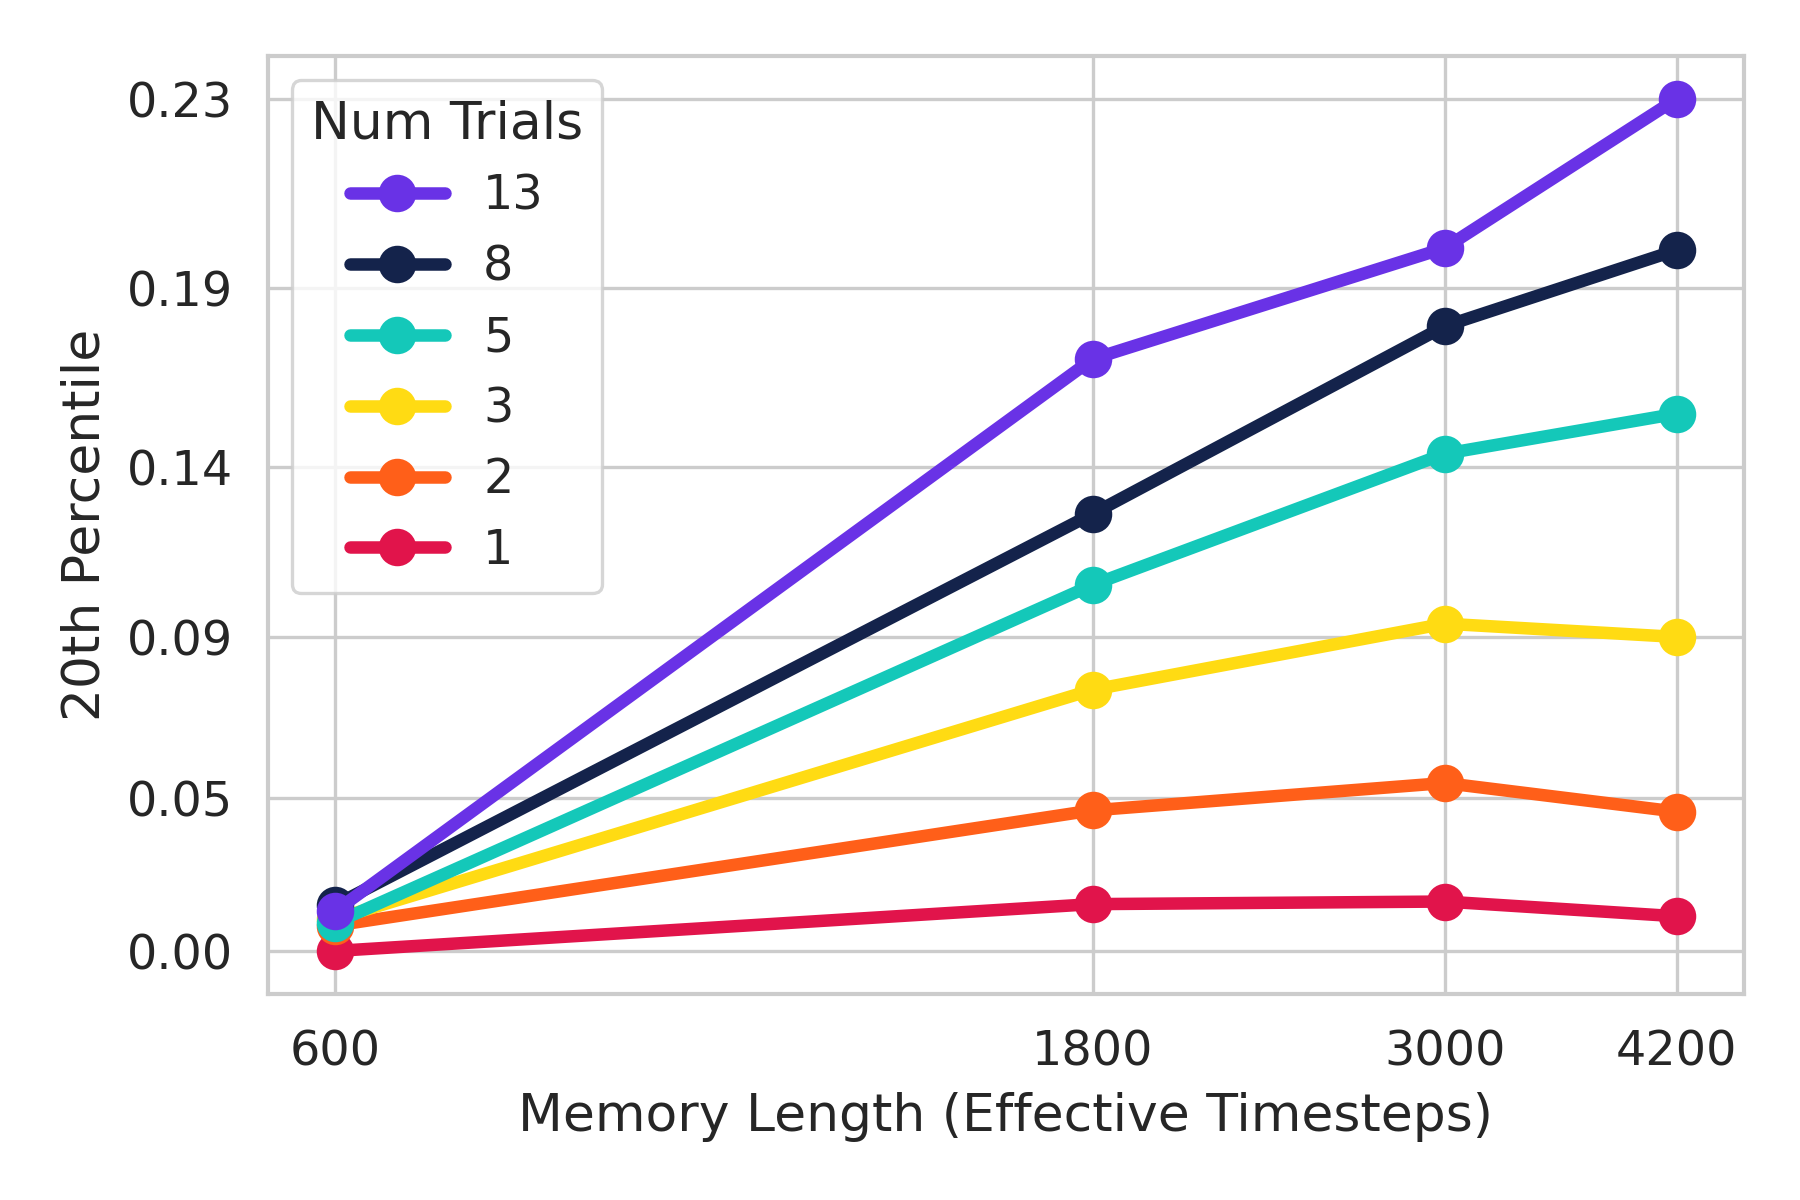
\includegraphics[width=\linewidth]{figures/scaling/memory_scaling_25g_steps_percentile20_log_log_memory.png}
        \vskip -3pt \caption{}
        \label{figure:scaling_memory_20th}
    \end{subfigure}
    \caption{Scaling Transformer-XL memory length increases 
    both median \textbf{(a)} and 20th percentile \textbf{(b)} test score. Both axes are log-scaled, according to the functions $\log(x)$ and $-\log(1-y)$, respectively, and the relationship between memory length and performance appears roughly linear on this scale. The slope is steeper when evaluating higher numbers of trials, showing that scaling the memory is particularly effective at encouraging stronger few-shot adaptation.}
\label{figure:scaling_memory}
\end{figure}

Appendix \ref{app:network-scaling} details the computational costs of the various model sizes, and shows FLOPs adjusted results. While larger models do indeed have better zero-shot score and adaptation than smaller ones for the same number of training steps, and are more sample efficient, the biggest model may not always be the best choice when compute cost is taken into account.

\paragraph{Scaling memory length.}

Performance also scales with the length of AdA's memory. The experimental setting is shown in Table \ref{tab:memory-scaling}, where we examine the number of previous network activations we cache, investigating values from $100$ to $700$, which, with $6$ Transformer-XL blocks, yields an effective timestep range of $600$ to $4200$ timesteps.\footnote{Transformer-XL enables the use of longer, variable-length context windows by concatenating a cached memory of previous attention layer inputs to the keys and values during each forward pass. Since inputs to intermediate layers are activations from the previous layer, which in themselves contain information about the past, caching $M$ activations theoretically allows for an effective memory horizon of $M \times L$, where $L$ is the number of attention layers in the network. } 

Figure \ref{figure:scaling_memory} shows that, as with model size, scaling memory length helps performance, especially in the lower test percentiles, pushing performance on the tails of the distribution. For any of our tasks, the maximum trial duration is 300 timesteps, so it is interesting that performance on, for example, $5$ trials ($1500$ timesteps) continues to increase for ``effective memory lengths'' between 1800 and 4200. This indicates that it is easier for the Transformer-XL to make use of explicitly given memory activations rather than relying on theoretically longer-range information implicit in those activations. 

